\avsnitt{Slutlig design}
Vi valde att dela upp v�rat projekt p� ett s�dant sett att det finns ett separat paket som heter \emph{cards} vilket �r t�nkt som ett allm�nt kortspels-paket med kort, kortlekar, spelare, h�nder osv och sedan ett paket, \emph{texasholdem}, som �r mer specifikt inriktat p� kortspelet Texas Holdem. I det senare ligger ocks� s�dant som mer styr spelregler och spelmekaniken.

Nedan �r ett klassdiagram �ver hela v�rt projekt:\\
\DeclareGraphicsExtensions{.png}
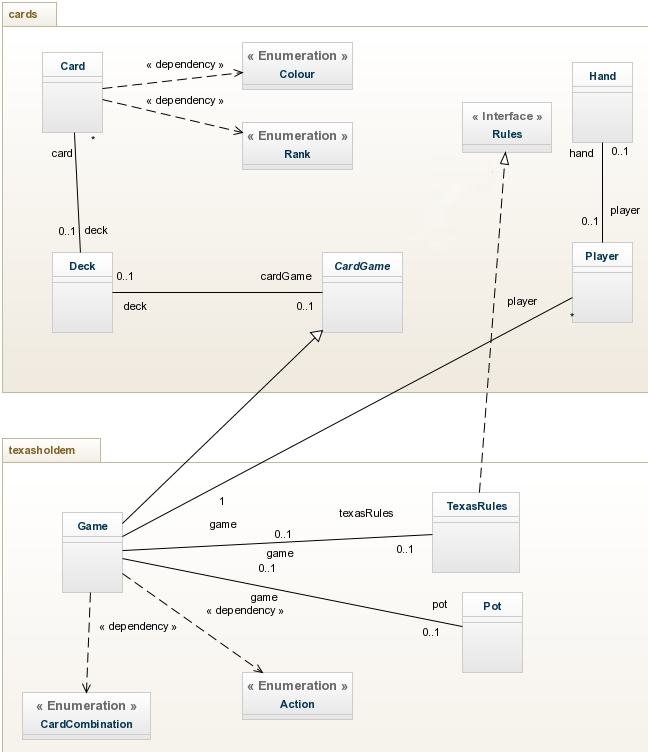
\includegraphics[natwidth=848, natheight=958, scale=0.73, angle=0, trim = 0mm 0mm 42mm 16mm]{bilder/diagram/klassdiagram-2014-10-28}

Samt n�gra mer detaljerade diagram �ver projektet;

\DeclareGraphicsExtensions{.png}
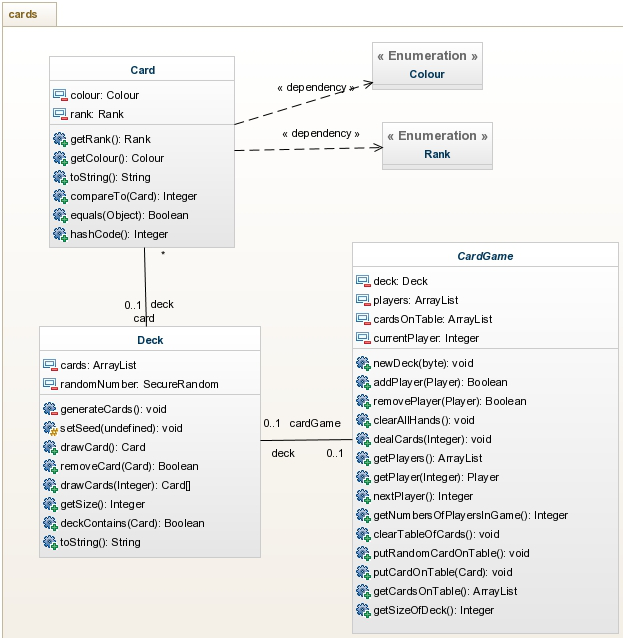
\includegraphics[natwidth=623, natheight=638, scale=0.91, angle=0, trim = 0mm 0mm 0mm 26mm]{bilder/diagram/card1}

\DeclareGraphicsExtensions{.png}
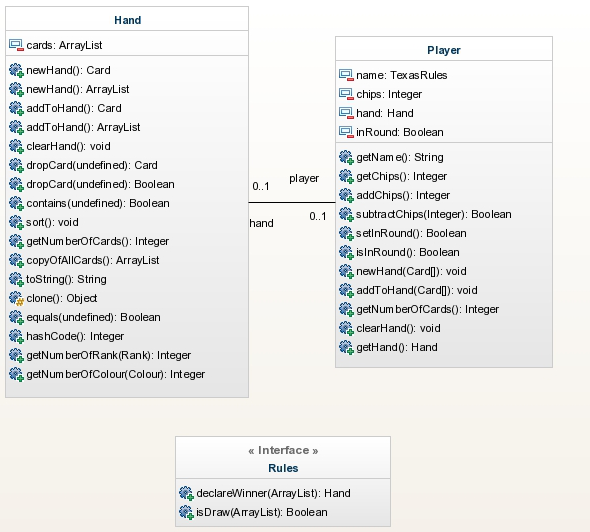
\includegraphics[natwidth=590, natheight=532, scale=0.95, angle=0, trim = 0mm 0mm 0mm 5mm]{bilder/diagram/card2}

\DeclareGraphicsExtensions{.png}
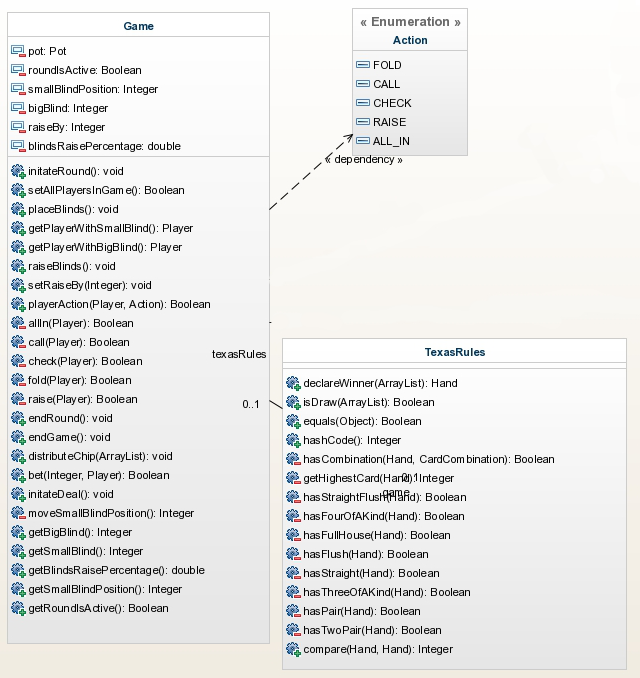
\includegraphics[natwidth=640, natheight=678, scale=0.84, angle=0, trim = 0mm 0mm 0mm 19mm]{bilder/diagram/texas1}

\DeclareGraphicsExtensions{.png}
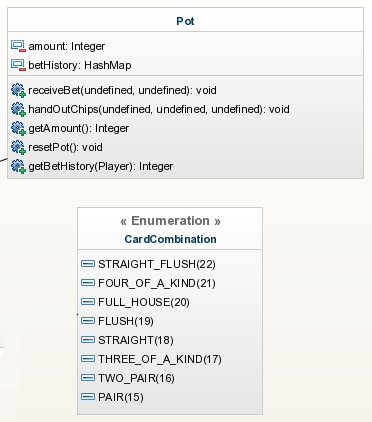
\includegraphics[natwidth=372, natheight=422, scale=1, angle=0, trim = 0mm 0mm 0mm 0mm]{bilder/diagram/texas2}
